%==============================================================================
\chapter{Fundamentos}\label{fundamentos}
%==============================================================================

Este trabalho é baseado em conceitos de aprendizado de máquina, que dedica-se na elaboraçãode algoritmos e técnicas que permitem um computador a aprender padrões.  

\section{Aprendizado de máquina}\label{sec:aprendizadodemaquina}

Para realizar a aprendizagem é necessário primeiramente dados de entrada que servem como exemplo para nosso modelo, com esses dados é possível treinar o modelo para que ele possa então aprender com base nesses exemplos para que depois seja possível generalizar sobre outros dados não testados ainda. O diagrama da \autoref{fig:passoapasso} abaixo mostra os passos para obter o resultado final.

\begin{figure}[htb]
	  \caption{Diagrama para resultado final}\label{fig:passoapasso}
	  \begin{center}
	      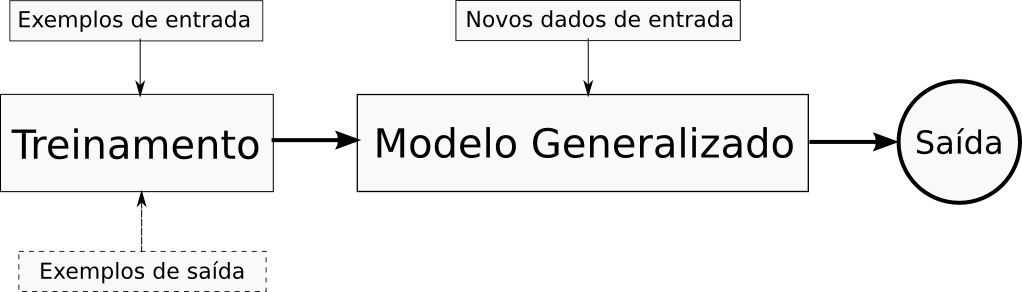
\includegraphics[scale=0.5]{img/passoapasso}
	  \end{center}
\end{figure}


O aprendizado de máquina pode ser dividido em duas abordagens: O \textbf{aprendizado supervisionado}, onde é dado um conjunto de dados de entrada e já se sabe como a saída deve parecer, tendo a ideia de que há uma relação entre a entrada e a saída; O \textbf{aprendizado não supervisionado}, que nos permite abordar problemas com pouca ou até nenhuma ideia de como os resultados devem parecer, nesse caso a caixa de exemplos de saída pode não existir.

Neste trabalho a abordagem utilizada vai ser o aprendizado supervisionado, pois já temos uma classe gramatical apropriada para cada palavra em seu contexto.

O aprendizado supervisionado permite dividir os problemas em duas categorias distintas:


\begin{itemize}
	\item \textbf{Regressão}: Tenta-se prever resultados com uma saída contínua, significando que estamos tentando mapear variáveis de entrada em alguma função contínua. A \autoref{fig:demregressao} demonstra esse processo. Nessa demonstração, os círculos em vermelho são dados de exemplo, já a reta azul representa a predição feita pela regressão.
	\item \textbf{Classificação}:  Tenta-se prever resultados em uma saída discreta, ou seja, estamos tentando mapear variáveis de entrada em categoriais discretas. A \autoref{fig:demclassificacao} demonstra esse processo. Aqui tem duas classes diferentes, as representadas pelos círculos amarelos e pelas cruzes vermelhas, já o contorno em verde representa o resultado da classificação sobre esses dados de exemplo.


	\textit{- falar mais sobre classificacao?} 

	\textit{- falar o que são features?}

	\textit{- mostrar matematicos (hipotese, custo, gradiente desc, probabilidades)?}

	\textit{- falar de exemplos reais?}


\end{itemize}


\begin{figure}[htb]
	  \caption{Demonstração de regressão}\label{fig:demregressao}
	  \begin{center}
	      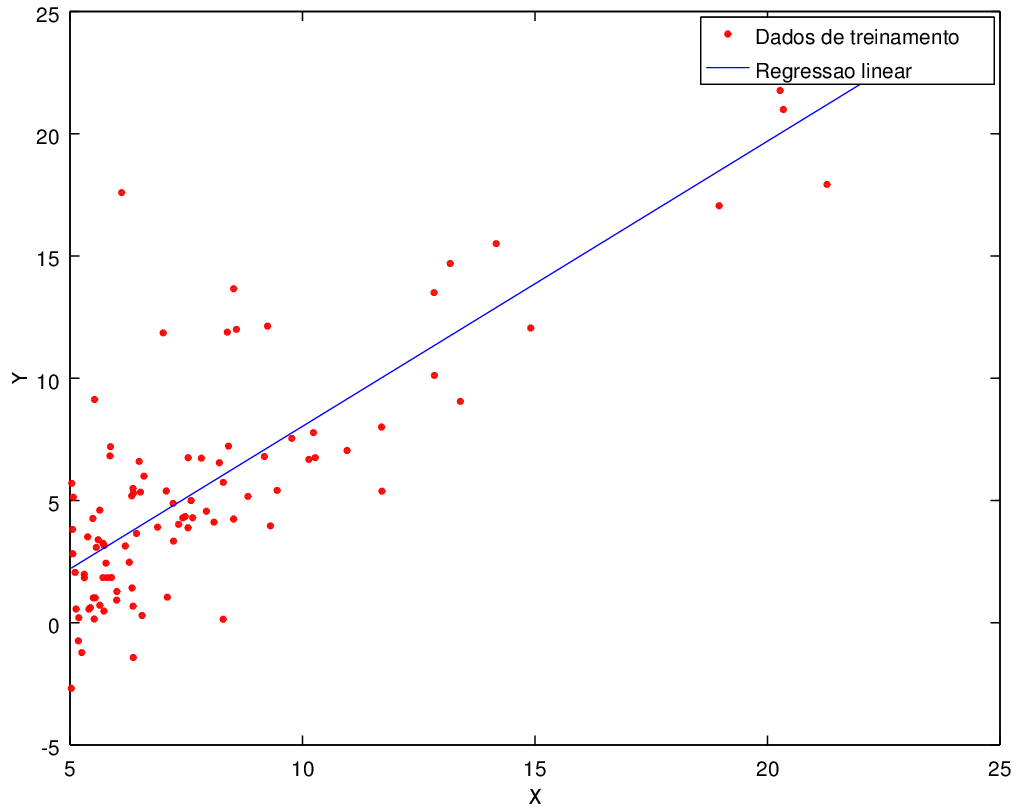
\includegraphics[scale=0.6]{img/regressao2}
	  \end{center}
\end{figure}

\begin{figure}[htb]
  \caption{Demonstração de classificação}\label{fig:demclassificacao}
  \begin{center}
      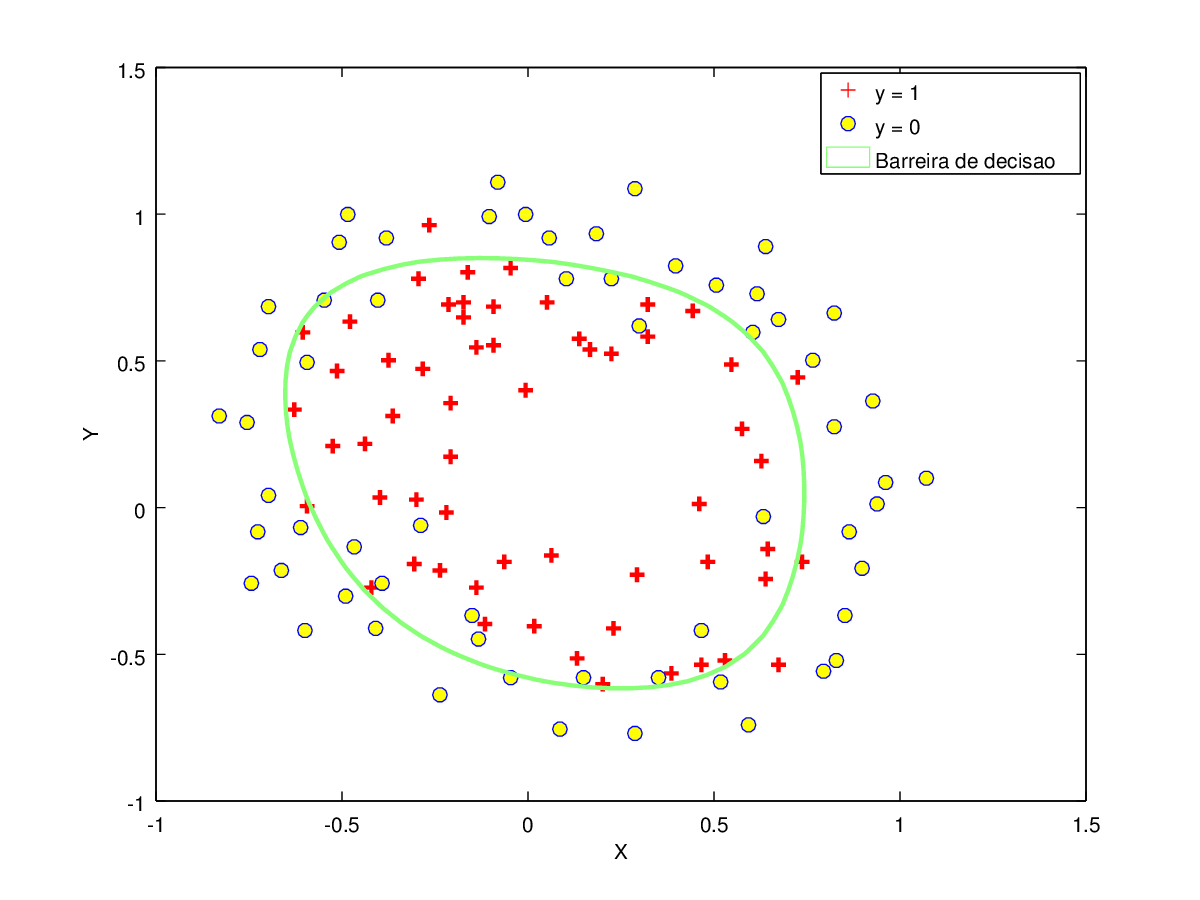
\includegraphics[scale=0.6]{img/classificacao2}
  \end{center}
\end{figure}


O POS tagging é um problema de classificação multiclasse, onde temos que etiquetar uma palavra em uma de várias categorias possíveis. É possível fazer isso ao dividir o problema em \textit{n + 1} problemas de classificação binária.



\section{Córpus e seu conjunto de classes gramaticais}

Córpus são uma coleção de textos colocados como um só, eles são os exemplos de entrada para nosso treinamento. A qualidade e o tamanho desses córpus são importantes para que o etiquetador possa generalizar sentenças ainda não vistas. Eles contém também um conjunto de classes gramaticais associadas a cada palavra.

Esses conjuntos podem se diferenciar na sua granularidade, como por exemplo, podem ter diferentes classes gramáticais para nomes no plural e no singular, ou agrupar eles em uma única classe [X]. No inglês, há vários córpus de qualidade que são amplamento utilizados, são o Penn Treebank tagset [X], CLAWS5 [X] e CLAWS7 [X].

Já no português esses córpus estão evoluindo com o tempo, embora muitos erros são encontrados neles [X], eles ainda são a melhor opção devido a seu tamanho e qualidade, os principais e mais utilizados para essa tarefa são o Mac-Morpho [X] com cerca de um milhão de palavras, que retrata artigos publicados na Folha de São Paulo em 1994. O Tycho Brahe [X] que também tem cerca de um milhão de palavras e retrata assuntos históricos de 66 textos diferentes, a linguagem utilizada nele é muito diferente da usada no cotidiano e por isso o seu uso é apenas a fim de curiosidade. Temos também o Bosque [X], que contém cerca de 185 mil palavras. Além desses, [X] et al. apresenta uma versão revisada do Mac-Morpho, com classes gramaticais novas e junção de outras. 

Infelizmente esses córpus não podem ser combinados em um só, já que eles se diferenciam no conjunto de classes gramaticais e também no seu uso associado.

A aprendizagem baseada em córpus tem se mostrado uma estratégia atrativa, já que pode ser usado recursos criados com melhores performance [X, Y, Z]. E nesse trabalho vamos utilizar três córpus que são o Mac-Morpho original; Mac-Morpho revisado e o Tycho Brahe. O conjunto de etiquetadas para esses córpus podem ser encontrados, respectivamente, em [X], [Y] e [Z].


\textit{- Falar mais alguma coisa sobre?}

\textit{- Colocar alguma tabela aqui?}



\section{Representação das palavras}

Palavras \footnote{Uma palavra pode ser qualquer conjunto de caracteres, inclusive pontuações, números, etc.} podem ser representadas de várias maneiras em um modelo de aprendizagem, podendo ser até mesmo feito o uso real da palavra como um conjunto de caracteres.

No entanto, a melhor abordagem e a mais indicada atualmente é a utilização de \textit{word embeddings} [X], elas são representação de palavras como vetores reais valorados em um espaço multidimensional [X]. Elas podem ser geradas de maneiras diferentes, dependendo da técnica utilizada, clássicas abordagens baseiam-se na frequência e co-ocorrência [X] das palavras, até mesmo via modelos de redes neurais [X].

Ao 


\section{Redes neurais profundas}